
 \FloatBarrier

\section{Maximization problems}\label{sec:maximization}




The evolutionary dynamics can be used to solve convex optimization problems. 
We can use the properties of population games to design games that maximize some function $f(\bs{z})$, where $\bs{z}\in\mathbb{R}^{n}$ is a vector of $n$ variables, i.e., $\bs{z} = [z_1, \ldots, z_k, \ldots, z_n]$. Below we show two alternatives to solve this optimization problem using either a single population or $n$ populations.



\subsection{Single Population Case}

First, let us consider a population where each agent can choose one of the $n+1$ strategies. In this case, the first $n$ strategies correspond one variable of the objective function and the $n+1\th$ strategy can be seen as a slack variable. 
Thus, $x_k$ is the proportion of agents that use the $k\th$ strategy, and it corresponds to the $k\th$ variable, i.e., $x_k = z_k$.
We define the fitness function of the $k\th$ strategy $F_k$ as the derivative of the objective function with respect to the $k\th$ variable, thus, $F_k(\bs{x}) \equiv \frac{\partial }{\partial x_k} f(\bs{x})$.

Note that if $f(\bs{x})$ is a concave function, then its gradient is a decreasing function. 
Recall that users attempt to increase their fitness by adopting the most profitable strategy in the population, say the $k\th$ strategy. This lead to an increase of $x_k$, which in turns decrease the fitness  $F_k(\bs{x})$. 

Furthermore, the equilibrium is reached when all agents that belong to the same population have the same fitness.
Thus, at the equilibrium $F_i(\bs{x}) = F_j(\bs{x})$, where $i,j\in\{1, \ldots, n \}$.
If we define $F_{n+1}(\bs{x}) = 0$, then at the equilibrium we have $F_i(\bs{x}) = 0$  for every strategy $i\in\{1, \ldots, n\}$. 
%
Since the fitness function decreases with the action of users, we can conclude that the strategy of the population evolves to make the gradient of the objective function equal to zero (or as close as possible). This resembles a gradient method to solve optimization problems.

% A characteristic of this implementation is that the  function of users depends on their strategy. Specifically, there are $n+1$ different strategy functions. 

Recall that the he evolution of the strategies lies in the simplex, that is, $\sum_{i \in S^p} z_i = m$. Hence, this implementation solves the following optimization problem:
\begin{equation}
\begin{aligned}
& \underset{\bs{z}}{\text{maximize}}
& &  f(\bs{z}) \\
& \text{subject to}
& & \sum_{i=1}^n z_i \leq m,
\end{aligned}
\label{eq:opt_problem}
\end{equation}
where m is the total mass of the population.
%Next we present a different implementation in which each user of the same population has the same fitness function.
%
Figure \ref{fig:maximization_a} shows an example of the setting described above for the  function
\begin{equation}\label{eq:objective_f}
 f(\bs{z}) = - (z_1-5)^2 - (z_2-5)^2.
\end{equation}
The simulation is executed during $0.6$ time units. 

\begin{figure}[htb]
\centering
 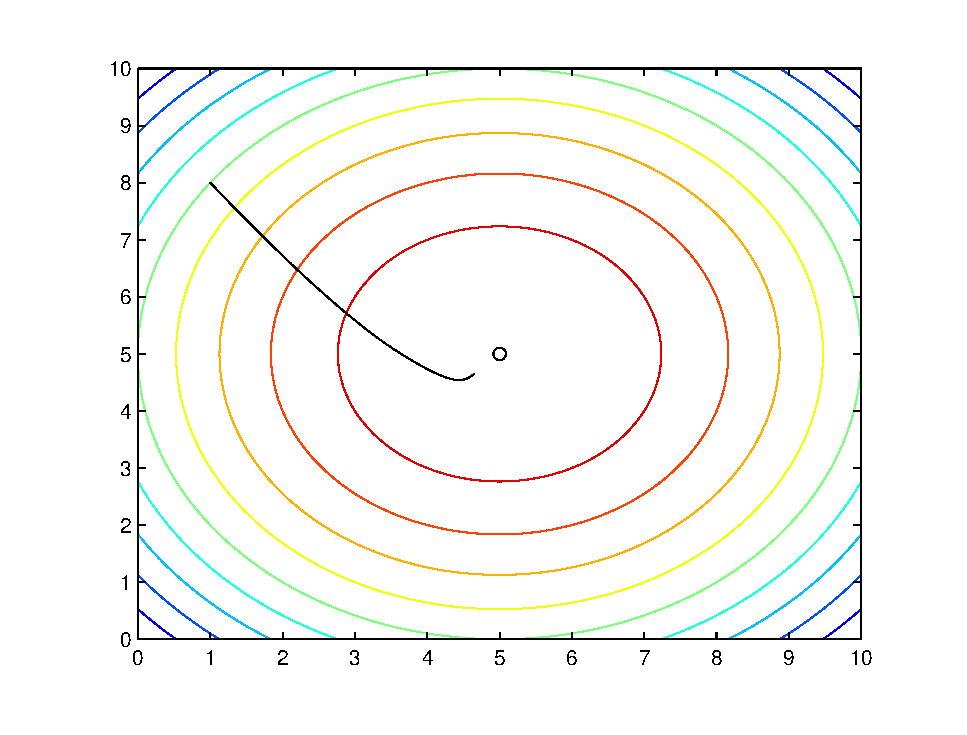
\includegraphics[width=.5\textwidth]{./images/maximization_a.eps}
 \caption{Evolution of the maximization setting using only one population.}
 \label{fig:maximization_a}
\end{figure}



\subsection{Multi-population Case}



Let us consider $n$ populations where each agent can choose one of two strategies. 
We define a population per each variable of the maximization problem and also $n$ additional strategies that resemble slack variables.
Thus, $x_i^p$ is the proportion of agents that use the $i\th$ strategy in the $p\th$ population. In this case $x_1^k$ corresponds to the $k\th$ variable, that is, $x_1^k = z_k$, while $x_2^k$ is a slack variable.
%
The fitness function $F_1^k$ of the $k\th$ population is defined as the derivative of the objective function with respect to the $k\th$ variable, that is, $F_1^k(\bs{x}) \equiv \frac{\partial }{\partial x_1^k} f(\bs{x})$. On the other hand, $F_2^k(\bs{x}) = 0$.
This implementation solves the following optimization problem:
\begin{equation}
\begin{aligned}
& \underset{\bs{z}}{\text{maximize}}
& &  f(\bs{z}) \\
& \text{subject to}
& & z_i \leq m^i, i =\{1,\ldots,n\}.
\end{aligned}
\label{eq:opt_problem}
\end{equation}


Figure \ref{fig:maximization_b} shows an example of the setting described above for the function in Eq. (\ref{eq:objective_f}).
The simulation is executed during $0.6$ time units. Note that the implementation using multiple populations reach the optimal value faster than the single population implementation.
\begin{figure}[htb]
\centering
 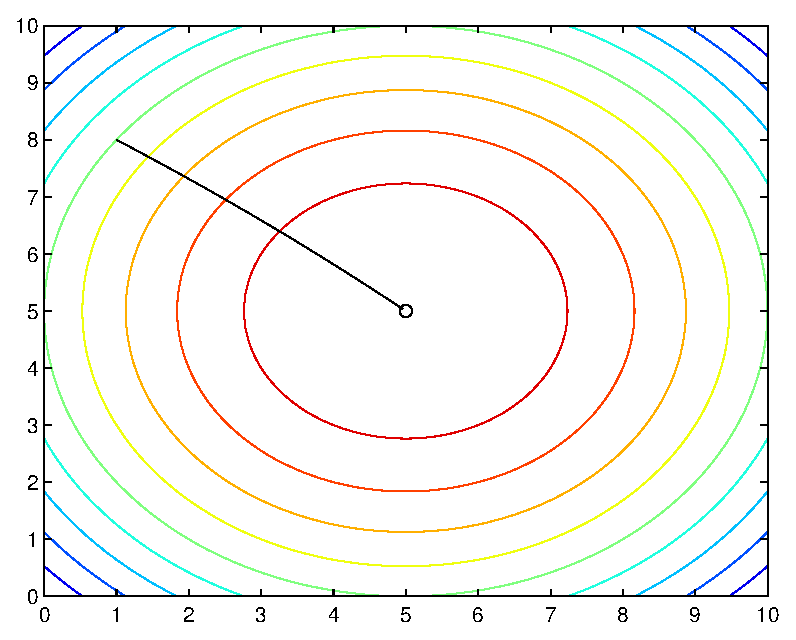
\includegraphics[width=.5\textwidth]{./images/maximization_b.eps}
 \caption{Evolution of the the maximization setting using $n$ populations.}
 \label{fig:maximization_b}
\end{figure}


The speed of convergence to the optimum depends on the dynamics and their parameters. For instance, we observed that the equilibrium of the BNN dynamics might be closer to the optimal solution $\bs{z}^*$ if the mass of the population $m^p$ is close to $\sum_{i=1}^N z_i$. Note that close to the optimum $\hat{F}^p$ is small, and if $m^p$ is too large, then the slack variable, such as  $x_2^k$, might be too large, making $x_1^k$ small. These conditions might hinder the convergence to the optimum because updates in the strategies are too small.